\documentclass{article}

% Packages required to support encoding
\usepackage{ucs}
\usepackage[utf8x]{inputenc}
\usepackage{graphicx} 
% Packages required by code

% Packages always used
\usepackage{listings}
\usepackage{hyperref}
\usepackage{xspace}
\usepackage[usenames,dvipsnames]{color}
\hypersetup{colorlinks=true,urlcolor=blue}


\usepackage[framed,numbered,autolinebreaks,useliterate] {mcode}


\usepackage{geometry}
\geometry{letterpaper,textwidth=350pt,textheight=680pt,tmargin=60pt,
            left=72pt,footskip=24pt,headsep=18pt,headheight=14pt}
\usepackage{amsmath}
\usepackage{amssymb}
\usepackage{textcase}
\usepackage{soul}

\newcommand{\mat}[1]{\boldsymbol{#1}}\renewcommand{\vec}[1]{\boldsymbol{\mathrm{#1}}}
\newcommand{\vecalt}[1]{\boldsymbol{#1}}

\newcommand{\conj}[1]{\overline{#1}}

\newcommand{\normof}[1]{\|#1\|}
\newcommand{\onormof}[2]{\|#1\|_{#2}}

\newcommand{\itr}[2]{#1^{(#2)}}
\newcommand{\itn}[1]{^{(#1)}}

\newcommand{\eps}{\varepsilon}
\newcommand{\kron}{\otimes}

\DeclareMathOperator{\diag}{diag}
\DeclareMathOperator{\trace}{trace}
\DeclareMathOperator{\tvec}{vec}

\newcommand{\prob}{\mathbb{P}}
\newcommand{\probof}[1]{\prob\left\{ #1 \right\}}

\newcommand{\pmat}[1]{\begin{pmatrix} #1 \end{pmatrix}}
\newcommand{\bmat}[1]{\begin{bmatrix} #1 \end{bmatrix}}
\newcommand{\spmat}[1]{\left(\begin{smallmatrix} #1 \end{smallmatrix}\right)}
\newcommand{\sbmat}[1]{\left[\begin{smallmatrix} #1 \end{smallmatrix}\right]}

\newcommand{\RR}{\mathbb{R}}
\newcommand{\CC}{\mathbb{C}}

\providecommand{\eye}{\mat{I}}
\providecommand{\mA}{\ensuremath{\mat{A}}}
\providecommand{\mB}{\ensuremath{\mat{B}}}
\providecommand{\mC}{\ensuremath{\mat{C}}}
\providecommand{\mD}{\ensuremath{\mat{D}}}
\providecommand{\mE}{\ensuremath{\mat{E}}}
\providecommand{\mF}{\ensuremath{\mat{F}}}
\providecommand{\mG}{\ensuremath{\mat{G}}}
\providecommand{\mH}{\ensuremath{\mat{H}}}
\providecommand{\mI}{\ensuremath{\mat{I}}}
\providecommand{\mJ}{\ensuremath{\mat{J}}}
\providecommand{\mK}{\ensuremath{\mat{K}}}
\providecommand{\mL}{\ensuremath{\mat{L}}}
\providecommand{\mM}{\ensuremath{\mat{M}}}
\providecommand{\mN}{\ensuremath{\mat{N}}}
\providecommand{\mO}{\ensuremath{\mat{O}}}
\providecommand{\mP}{\ensuremath{\mat{P}}}
\providecommand{\mQ}{\ensuremath{\mat{Q}}}
\providecommand{\mR}{\ensuremath{\mat{R}}}
\providecommand{\mS}{\ensuremath{\mat{S}}}
\providecommand{\mT}{\ensuremath{\mat{T}}}
\providecommand{\mU}{\ensuremath{\mat{U}}}
\providecommand{\mV}{\ensuremath{\mat{V}}}
\providecommand{\mW}{\ensuremath{\mat{W}}}
\providecommand{\mX}{\ensuremath{\mat{X}}}
\providecommand{\mY}{\ensuremath{\mat{Y}}}
\providecommand{\mZ}{\ensuremath{\mat{Z}}}
\providecommand{\mLambda}{\ensuremath{\mat{\Lambda}}}
\providecommand{\mPbar}{\bar{\mP}}

\providecommand{\ones}{\vec{e}}
\providecommand{\va}{\ensuremath{\vec{a}}}
\providecommand{\vb}{\ensuremath{\vec{b}}}
\providecommand{\vc}{\ensuremath{\vec{c}}}
\providecommand{\vd}{\ensuremath{\vec{d}}}
\providecommand{\ve}{\ensuremath{\vec{e}}}
\providecommand{\vf}{\ensuremath{\vec{f}}}
\providecommand{\vg}{\ensuremath{\vec{g}}}
\providecommand{\vh}{\ensuremath{\vec{h}}}
\providecommand{\vi}{\ensuremath{\vec{i}}}
\providecommand{\vj}{\ensuremath{\vec{j}}}
\providecommand{\vk}{\ensuremath{\vec{k}}}
\providecommand{\vl}{\ensuremath{\vec{l}}}
\providecommand{\vm}{\ensuremath{\vec{l}}}
\providecommand{\vn}{\ensuremath{\vec{n}}}
\providecommand{\vo}{\ensuremath{\vec{o}}}
\providecommand{\vp}{\ensuremath{\vec{p}}}
\providecommand{\vq}{\ensuremath{\vec{q}}}
\providecommand{\vr}{\ensuremath{\vec{r}}}
\providecommand{\vs}{\ensuremath{\vec{s}}}
\providecommand{\vt}{\ensuremath{\vec{t}}}
\providecommand{\vu}{\ensuremath{\vec{u}}}
\providecommand{\vv}{\ensuremath{\vec{v}}}
\providecommand{\vw}{\ensuremath{\vec{w}}}
\providecommand{\vx}{\ensuremath{\vec{x}}}
\providecommand{\vy}{\ensuremath{\vec{y}}}
\providecommand{\vz}{\ensuremath{\vec{z}}}
\providecommand{\vpi}{\ensuremath{\vecalt{\pi}}}

\sodef\allcapsspacing{\upshape}{0.15em}{0.65em}{0.6em}%

\makeatletter
\def\maketitle{%
\par
\hrule height 0.75pt\vspace{1ex}
\par\noindent
\begin{minipage}{0.5\textwidth}
\scshape
purdue university $\cdot$ CS 580 \\
Introduction to the Analysis of Algorithms
\end{minipage}
\begin{minipage}{0.5\textwidth}
\raggedleft
\MakeTextUppercase{\allcapsspacing{\@title}}\\[0.2ex]
\textit{\@author}\\[0.2ex]
\textit{\@date}
\end{minipage}
\par\vspace{1ex}
\hrule height 1pt
\vspace{2ex}
\par
}
\makeatother

\author{Jun Cheng}
\title{Lecture Notes}
% auto generate a title
\AtBeginDocument{\maketitle}


\title{Homework}



\begin{document} 



\hypertarget{}{}
\subsection*{{Problem 0: Homework checklist}}
\label{problem_0_homework_checklist_2}

\checkmark	I didn't talk with any one about this homework. \newline
\checkmark 	Source-code are included at the end of this document. 


\hypertarget{}{}
\subsection*{{Problem 1: Prove or disprove}}
\label{}
\begin{enumerate} 
\item 
False.  The eigenvalues of an $n\times n$ real-valued matrix are not always real. For example, 
\begin{align*} 
\mA &=\bmat{cos\theta & -sin\theta \\ sin\theta & cos\theta}\\
\lambda_1 &= cos\theta+i\sin\theta \\
\lambda_2 &= cos\theta-i\sin\theta \\
\end{align*}

\item 
True. 
\begin{align*} 
det(\mA^T\mA+\gamma\mI)\neq 0
\end{align*}
So the solution to $(\mA^T\mA+\gamma\mI)\vx=\vb$ is unique for any $\gamma>0$. 
\item 
True. 
Suppose that $\alpha\neq 0$ is not an eigenvalue of $\mA$. Then 
\begin{align*}
(\mA-\alpha\mI)\vv\neq 0 \\ 
\end{align*}
So $\mA-\alpha\mI$ is non-singular. \\
Then $\alpha\mI$ and $\mA=(\mA-\alpha\mI) + \alpha\mI$ are non-singular matrices. 

\item 
False. An symmetric matrix has an orthogonal set of eigenvector. 
\begin{align*} 
\mA &=\bmat{2 & -4 \\ -1 & -1}\\
\lambda_1 &= 3 \\
\lambda_2 &= -2 \\
\vv_1=\bmat{0.9701 \\ -0.2425}\\
\vv_2=\bmat{0.7071 \\ 0.7071}
\end{align*}
Those two eigenvectors are not orthogonal. 

\end{enumerate} 


\hypertarget{}{}
\subsection*{{Problem 2: The power method, and beyond!}}
\label{}
\begin{enumerate} 
\item 
Based on the definition of eigenvalue: \\
\begin{align*} 
\mA\vx& = \lambda\vx \\
\mA\vx^{(i)} &=\lambda^{(i)}\vx^{(i)}
\end{align*}
Then 
\begin{align*} 
\lambda &= \frac{\vx^T\mA\vx}{\vx^T\vx} \\
\lambda^{(i)} &= \frac{\vx^{(i)T}\mA\vx^{(i)}}{\vx^{(i)T}\vx^{(i)}} \\
|\lambda-\lambda^{(i)}| &= |  \frac{\vx^T\mA\vx}{\vx^T\vx} - \frac{\vx^{(i)T}\mA\vx^{(i)}}{\vx^{(i)T}\vx^{(i)}}|
& = |(\vx-\vx^{(i)})^T(\vx-\vx^{(i)})|+ O(\epsilon^3)| \\
& = |\|\vx-\vx^{(i)}\|^2 +O(\epsilon^3)| \\
& = |\epsilon^2+O(\epsilon^3)| \\
& = O(\epsilon^2) 
\end{align*}
\item 
\begin{align*} 
\mA\vv & = \lambda\vv \\
\mA^{-1}\mA\vv & =\lambda\mA^{-1}\vv \\
\mA^{-1}\vv &=\frac{1}{\lambda}\vv
\end{align*}
Therefore the eigenvalues are $\frac{1}{\lambda} $. 

\item 
It doesn't converge.  The 'difference vs iterations' plot shows it does not converge to 0. \\
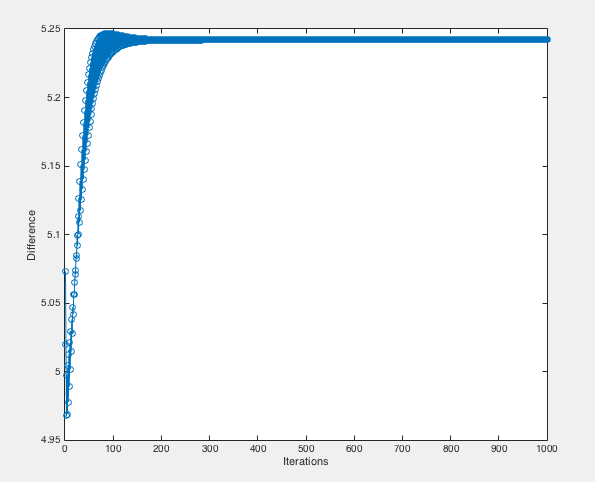
\includegraphics[width=0.7\textwidth]{problem2_3} 
%\centering 


\item  
If $\vv^{(k)} $is close to an eigenvector, then \\
\begin{align*} 
\|\vv^{(k)}-(\pm q_J)\| &\leq \epsilon \\
|\lambda^{(k)}-\lambda_J | &=O(\epsilon^2)
\end{align*}
Then one step of inverse iteration then gives: \\
\begin{align*} 
\|\vv^{(k+1)}-\vq_{J}\| = O(|\lambda^{(k)}-\lambda_J |\|\vv^{(k)}-\vq_{J}\|) = O(\epsilon^3)
\end{align*}

\item 
The code is list below: \\ 
\begin{verbatim} 
maxit = 20; 
dim = 6; 
A = rand(dim); 
A = A*A; 
e = abs(eig(A)); 
lamda = max(e); 
[V, D]  = eig(A); 
true_X = V(:,1) ; 
true_X = true_X/norm(true_X); 

x= rand(dim,1);
x= x/norm(x); 
lam = x'*A*x; 
diff = zeros(maxit,1); 
iter = zeros(maxit,1); 
eps = zeros(maxit,1); 
for i=1:maxit
    x=(A-lam*eye(size(A,1)))\x; 
    x = x/norm(x,2); 
    lam = x'*A*x; 
    diff(i) = norm(lam - lamda);  
    iter(i) = i; 
end
semilogy(iter, diff, 'o-') ; 
xlabel('Iterations'); 
ylabel('Difference'); 
\end{verbatim}
The result is plot below, and we can see the cubic convergence. \\
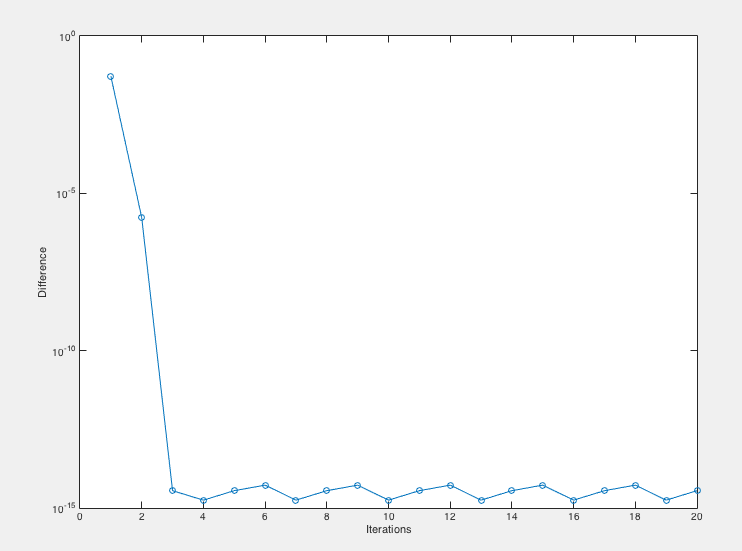
\includegraphics[width=0.7\textwidth]{problem2_4} 
\centering 

\end{enumerate} 


\hypertarget{}{}
\subsection*{{Problem 3: PageRank and the power method}}
\label{}
\begin{enumerate} 
\item 
\begin{align*}
\mM &=\mI-\alpha\mP \\
\mM^T &=\mI-\alpha\mP^T \\
\end{align*} 
Because the $\mP$ is a column-stochastic matrix, and then $\mP$ is a row-stochastic matrix.  
\begin{align*}
%\alpha<0 
1 &= \sum |\mP^T_{ij}| &   \\
\mP_{ii}  & = \sum_{i\neq} |\mP^T_{ij}| \\
\mM_{ii} & =  1-\alpha\mP_{ii}  \\
& = 1- \alpha\sum_{i\neq j} |\mP^T_{ij}| \\
\end{align*}
Because $\alpha<1$, then 
\begin{align*} 
|\mM^T_{ii}|>\sum_{i\neq j} |\mM^T_{ij}|
\end{align*}
Then$\mM_T$ is strictly diagonally dominant. We know that a strictly diagonally dominant matrix is nonsingular. 

\item 
Because $\vv$ is a non-negative vector whose elements sum to 1. \\
\begin{align*} 
\vv\ve^T\vv &= \bmat{v_1(v_1+v_2+...) \\ v_2(v_1+v_2+...) \\ ... 
\\ ... \\v_n(v_1+v_2+...)} \\
& = \vv \\
\mM\vv &= [\alpha\mP+(1-\alpha)\vv\ve^T]\vv  \\
&= \alpha\mP\vv + (1-\alpha)\vv\ve^T\vv \\
& =  \alpha\mP\vv + (1-\alpha)\vv \\
& = \alpha\bmat{\sum P_{1j} v_j\\ \sum P_{2j}v_j \\ ... \\ ... \\ \sum P_{nj} v_j} + (1-\alpha)\vv \\
\vx^1 &=\mM\vv  \\
\|\vv\|_1 &= \|\mM\vv\|_1 = \alpha\sum_{i}v_i[\sum_{j}P_{ji}] + (	1-\alpha) \\
& = 1
\end{align*}
For $ \vx^{(k+1)} = \mM\vx^{(k)} $, we always have $\|x^{(k+1)}\|_1 = 1$ \\


\item 
Suppose $\vx$ is the dominant eigenvector of matrix $\mM$  \\
\begin{align*} 
\mM\vx &= \vx \\
& = [\alpha\mP+(1-\alpha)\vv\ve^T]\vx \\ 
[\mI-(\alpha\mP+(1-\alpha)\vv\ve^T)]\vx=0 \\
\end{align*} 
We know that $\vv\ve^T\vx = \vx$ \\ 
Then \\
\begin{align*} 
(\mI-\alpha\mP^T)\vx-(1-\alpha)\vv & = 0 \\
 (\mI-\alpha\mP^T)\vx &= (1-\alpha)\vv
\end{align*}
\item 
The simplified iterations: \\
\begin{align*} 
\vx^{(k+1)} &= \alpha\mP\vx^{(k)} + (1-\alpha)\vv  \\
\vx  &= \alpha \mP\vx + (1-\alpha)\vv \\ 
\vx-\vx^{(k+1)} & = \alpha\mP\vx-\alpha\mP\vx^{(k)} \\
\|\vx-\vx^{(k+1)}\| &=\|\alpha\mP(\vx-\vx^{(k)}\|  \\
& = \|\alpha\mP\|\|\vx-\vx^{(k+1)} \|  \\
& \leq  \|\alpha\mP\| \|\alpha\mP\|...\|\vx-\vx^{(k-1)} \| \\
& \leq  \|\alpha\mP\|^{k+1}\|\vx-\vx^{(0)}\| \\
\end{align*} 
Therefore, the power method will converge to the solution of the linear system $ (\mI-\alpha\mP^T)\vx = (1-\alpha)\vv$. 

\item 
The first url shown is : 'http://aae.www.ecn.purdue.edu/' \\

\item 
$\vx(1)$ is $\vv(1)=[\frac{1}{n}, \frac{1}{n}, \frac{1}{n}... ]$ \\
Then the top 27 entries are : 
\begin{verbatim}
'http://aae.www.ecn.purdue.edu/'
    'http://aae.www.ecn.purdue.edu/AAE/'
    'http://aae.www.ecn.purdue.edu/AAE/Academic/'
    'http://aae.www.ecn.purdue.edu/AAE/Academic/Index.html'
    'http://aae.www.ecn.purdue.edu/AAE/Academic/New_Index.html'
    'http://aae.www.ecn.purdue.edu/AAE/Alumni/'
    'http://aae.www.ecn.purdue.edu/AAE/Alumni/97DEAPic.html'
    'http://aae.www.ecn.purdue.edu/AAE/Alumni/AlumniEvents.html'
    'http://aae.www.ecn.purdue.edu/AAE/Alumni/DEA.html'
    'http://aae.www.ecn.purdue.edu/AAE/Alumni/HonDoc.html'
    'http://aae.www.ecn.purdue.edu/AAE/Alumni/IndAdvisory.html'
    'http://aae.www.ecn.purdue.edu/AAE/Alumni/Index.html'
    'http://aae.www.ecn.purdue.edu/AAE/Alumni/New_Index.html'
    'http://aae.www.ecn.purdue.edu/AAE/Alumni/YourGift.html'
    'http://aae.www.ecn.purdue.edu/AAE/Alumni/industrialaffiliatesprogram.html'
    'http://aae.www.ecn.purdue.edu/AAE/Alumni/outstandingeng.html'
    'http://aae.www.ecn.purdue.edu/AAE/Alumni/williameboeing.html'
    'http://aae.www.ecn.purdue.edu/AAE/Astronaut/Armstrong.html'
    'http://aae.www.ecn.purdue.edu/AAE/Astronaut/Astronaut.html'
    'http://aae.www.ecn.purdue.edu/AAE/Astronaut/Blaha.html'
    'http://aae.www.ecn.purdue.edu/AAE/Astronaut/Bridges.html'
    'http://aae.www.ecn.purdue.edu/AAE/Astronaut/Brown.html'
    'http://aae.www.ecn.purdue.edu/AAE/Astronaut/Casper.html'
    'http://aae.www.ecn.purdue.edu/AAE/Astronaut/Cernan.html'
    'http://aae.www.ecn.purdue.edu/AAE/Astronaut/Chaffee.html'
    'http://aae.www.ecn.purdue.edu/AAE/Astronaut/Covey.html'
    'http://aae.www.ecn.purdue.edu/AAE/Astronaut/Gardner.html'
\end{verbatim}
\end{enumerate} 




\end{document}
